\section{The Electrical System}

The electrical system consists of two parts: the power distribution system and signals. Each will be discussed in the following sections. Wiring diagrams are provided in Appendix.

\subsection{The Power Distribution System}

\subsubsection{Power Supplies}
Power to the entire system comes from the 3-prong plug running through the PVC pipe fixtures on the driver's left side of the electronics box.

\begin{figure}[h!]
\centering
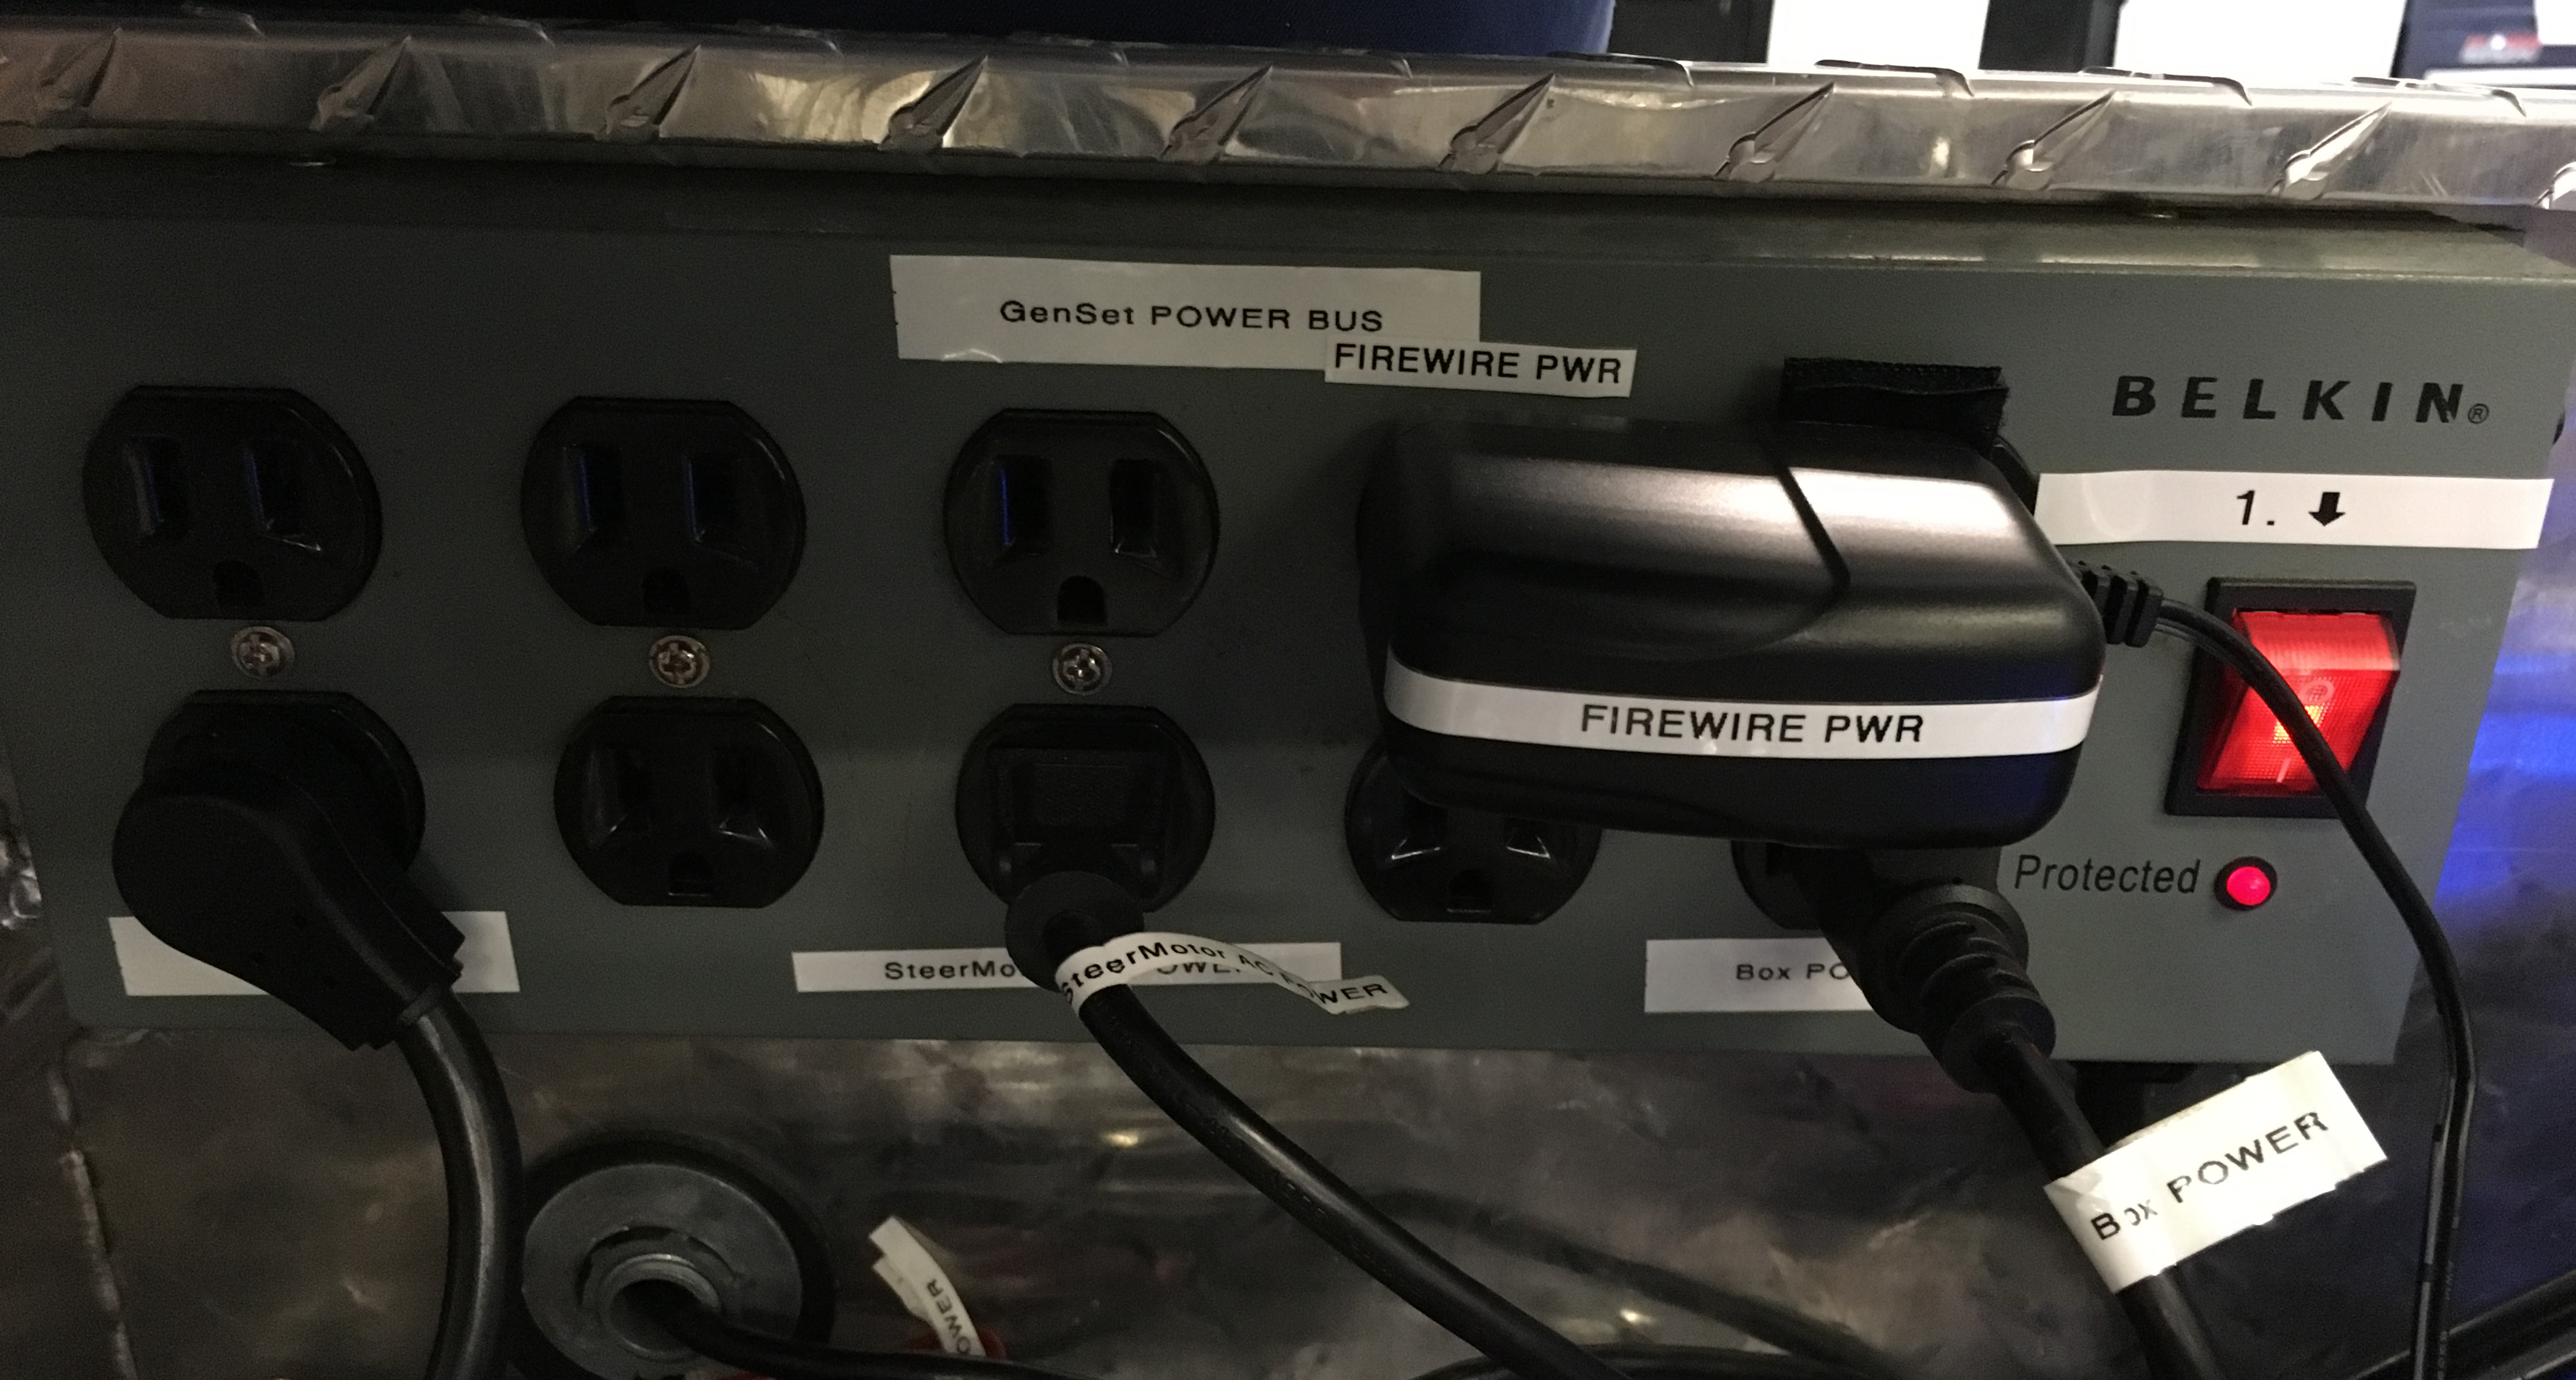
\includegraphics[scale=.1]{Photos/PowerStrip.jpg}
\caption{The power strip on the side of the electronics box}
\label{fig:powerstrip}
\end{figure} 

 \noindent The 3-prong plug attached to the power strip plugs into building power when the vehicle is in the Large Project Building and supplies power to the power strip mounted on the wall of the electronics box on the driver's left side. Alternatively, during operation, the 3-prong plug is plugged into a Honda EU2000i generator that should be mounted in the back of the vehicle:\\ \\
%
 Power to the rest of the system is then drawn from that power strip. The devices plugged into that power strip are shown in the diagram below:\\ \\

\begin{figure}[h!]
\centering
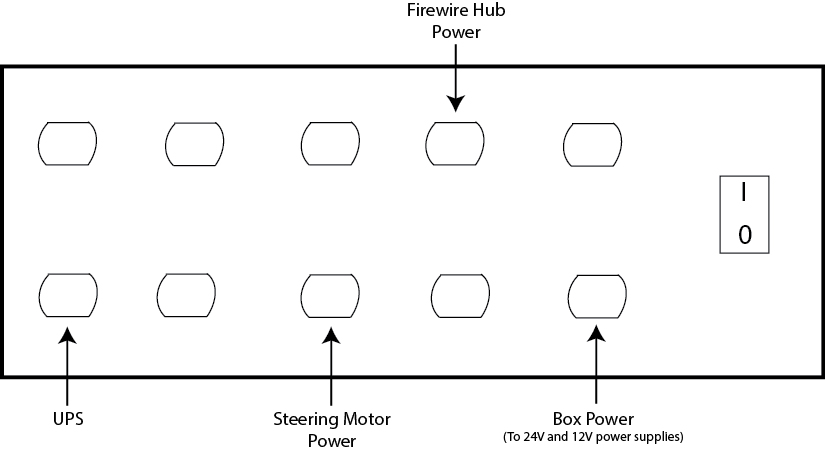
\includegraphics[scale=.6]{Photos/PowerStrip_Drawing.jpg}
\caption{Drawing of devices plugged into the power strip}
\label{fig:powerstripdrawing}
\end{figure} 

\noindent The entire system has 3 voltages that powers everything: 5 volts, 12 volts and 24 volts:
\begin{enumerate}
\item A Meanwell HRP-600-24 converts 120V AC power from the power strip to 24V DC power
\item A Meanwell HRP-300-12 converts 120V AC power from the power strip to 12V DC power
\item A Meanwell SB-15B-05 converts 24V DC power from the 24V DC power supply to 5V DC power
\end{enumerate}
%
The 24V and 12V power supplies are located on the lower deck of the electronics enclosure and the 5V power supply is located on the upper deck.

\newpage 

\subsubsection{Overview of Fuses}
There are 4 main fuse blocks used on the vehicle to distribute power via fuses to all electronic devices on board:
\begin{enumerate}
\item 1 Blue Sea Systems fuse block (C24) handles all 24V power distribution
\item 2 Blue Sea Systems fuse blocks (C12 and M12) handle all 12V power distribution
\item 1 linear fuse block handles all 5V power distribution 
\end{enumerate}
%
From the lower deck, three main power busses run to the upper deck: two 24V busses and one 12V bus. One 24V bus runs to the C24 fuse block and the other 24V bus runs to the 5V power supply that converts 24V DC power to 5V DC power. The 12V bus runs to the M12 fuse block. The C12 fuse block is powered from one of the outputs on the M12 fuse block.
%
\subsubsection{24V Power Distribution (C24 Fuse Block)}

\begin{minipage}{0.6\textwidth}
Five outputs on the C24 fuse block are used:\\
\begin{enumerate}
\item Signal to a 24V sensing probe
\item LIDAR power
\item LIDAR power
\item Navcomm GPS power
\item Safety light power
\end{enumerate}
\end{minipage} \hfill
\begin{minipage}{0.5\textwidth}
\begin{figure}[H]
\centering
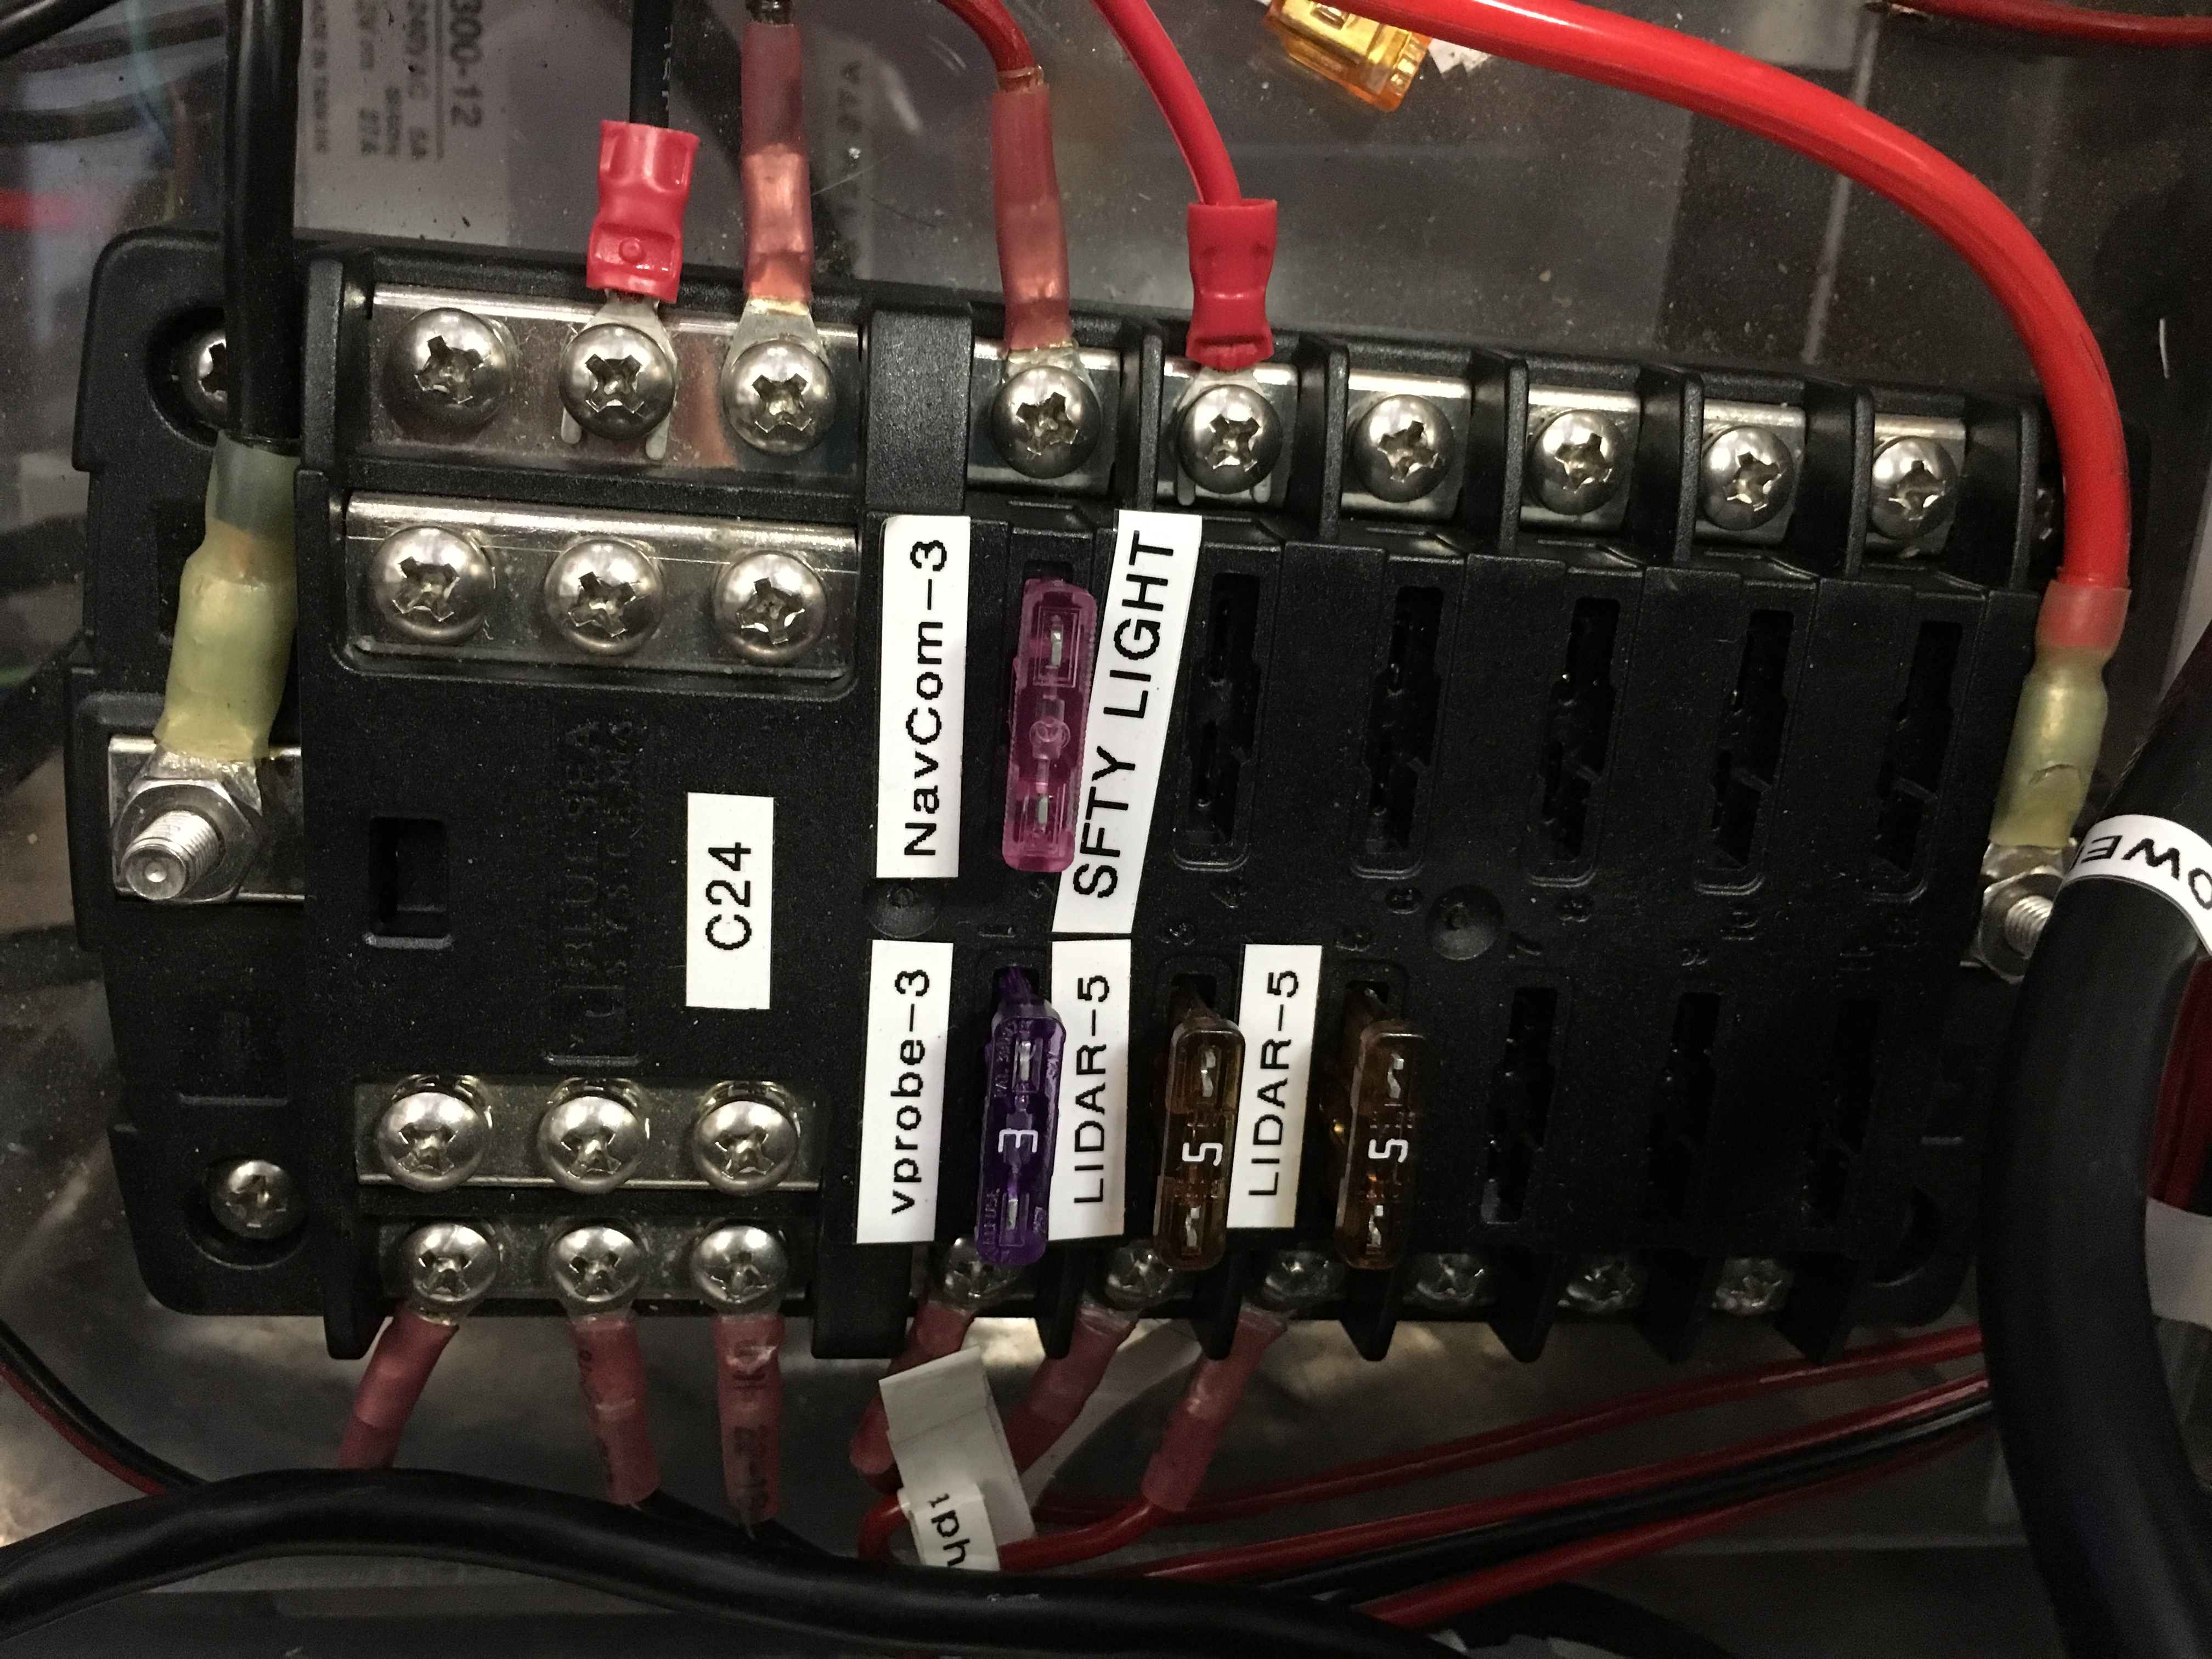
\includegraphics[scale=.05, angle=-90]{Photos/C24.jpg}
\caption{\label{fig:C24} C24 Fuse Block}
\end{figure}
\end{minipage}

\bigskip

\noindent  Except for the signal to the 24V sensing probe, all of the other 4 lines run to the appropriate equipment outside the electronics box. The signal to the 24V sensing probe runs to the voltage sense project box (discussed in a later subsection).

\newpage

\subsubsection{12V Power Distribution (C12 Fuse Block)}

\begin{minipage}{0.6\textwidth}
Five outputs on the C12 fuse block are used:
\begin{enumerate}
\item Power for the cab fans
\item Signal to a 12V sensing probe
\item INS power
\item Power for ethernet switch
\item E-Stop 12V power
\end{enumerate}
\end{minipage} \hfill
\begin{minipage}{0.5\textwidth}
\begin{figure}[H]
\centering
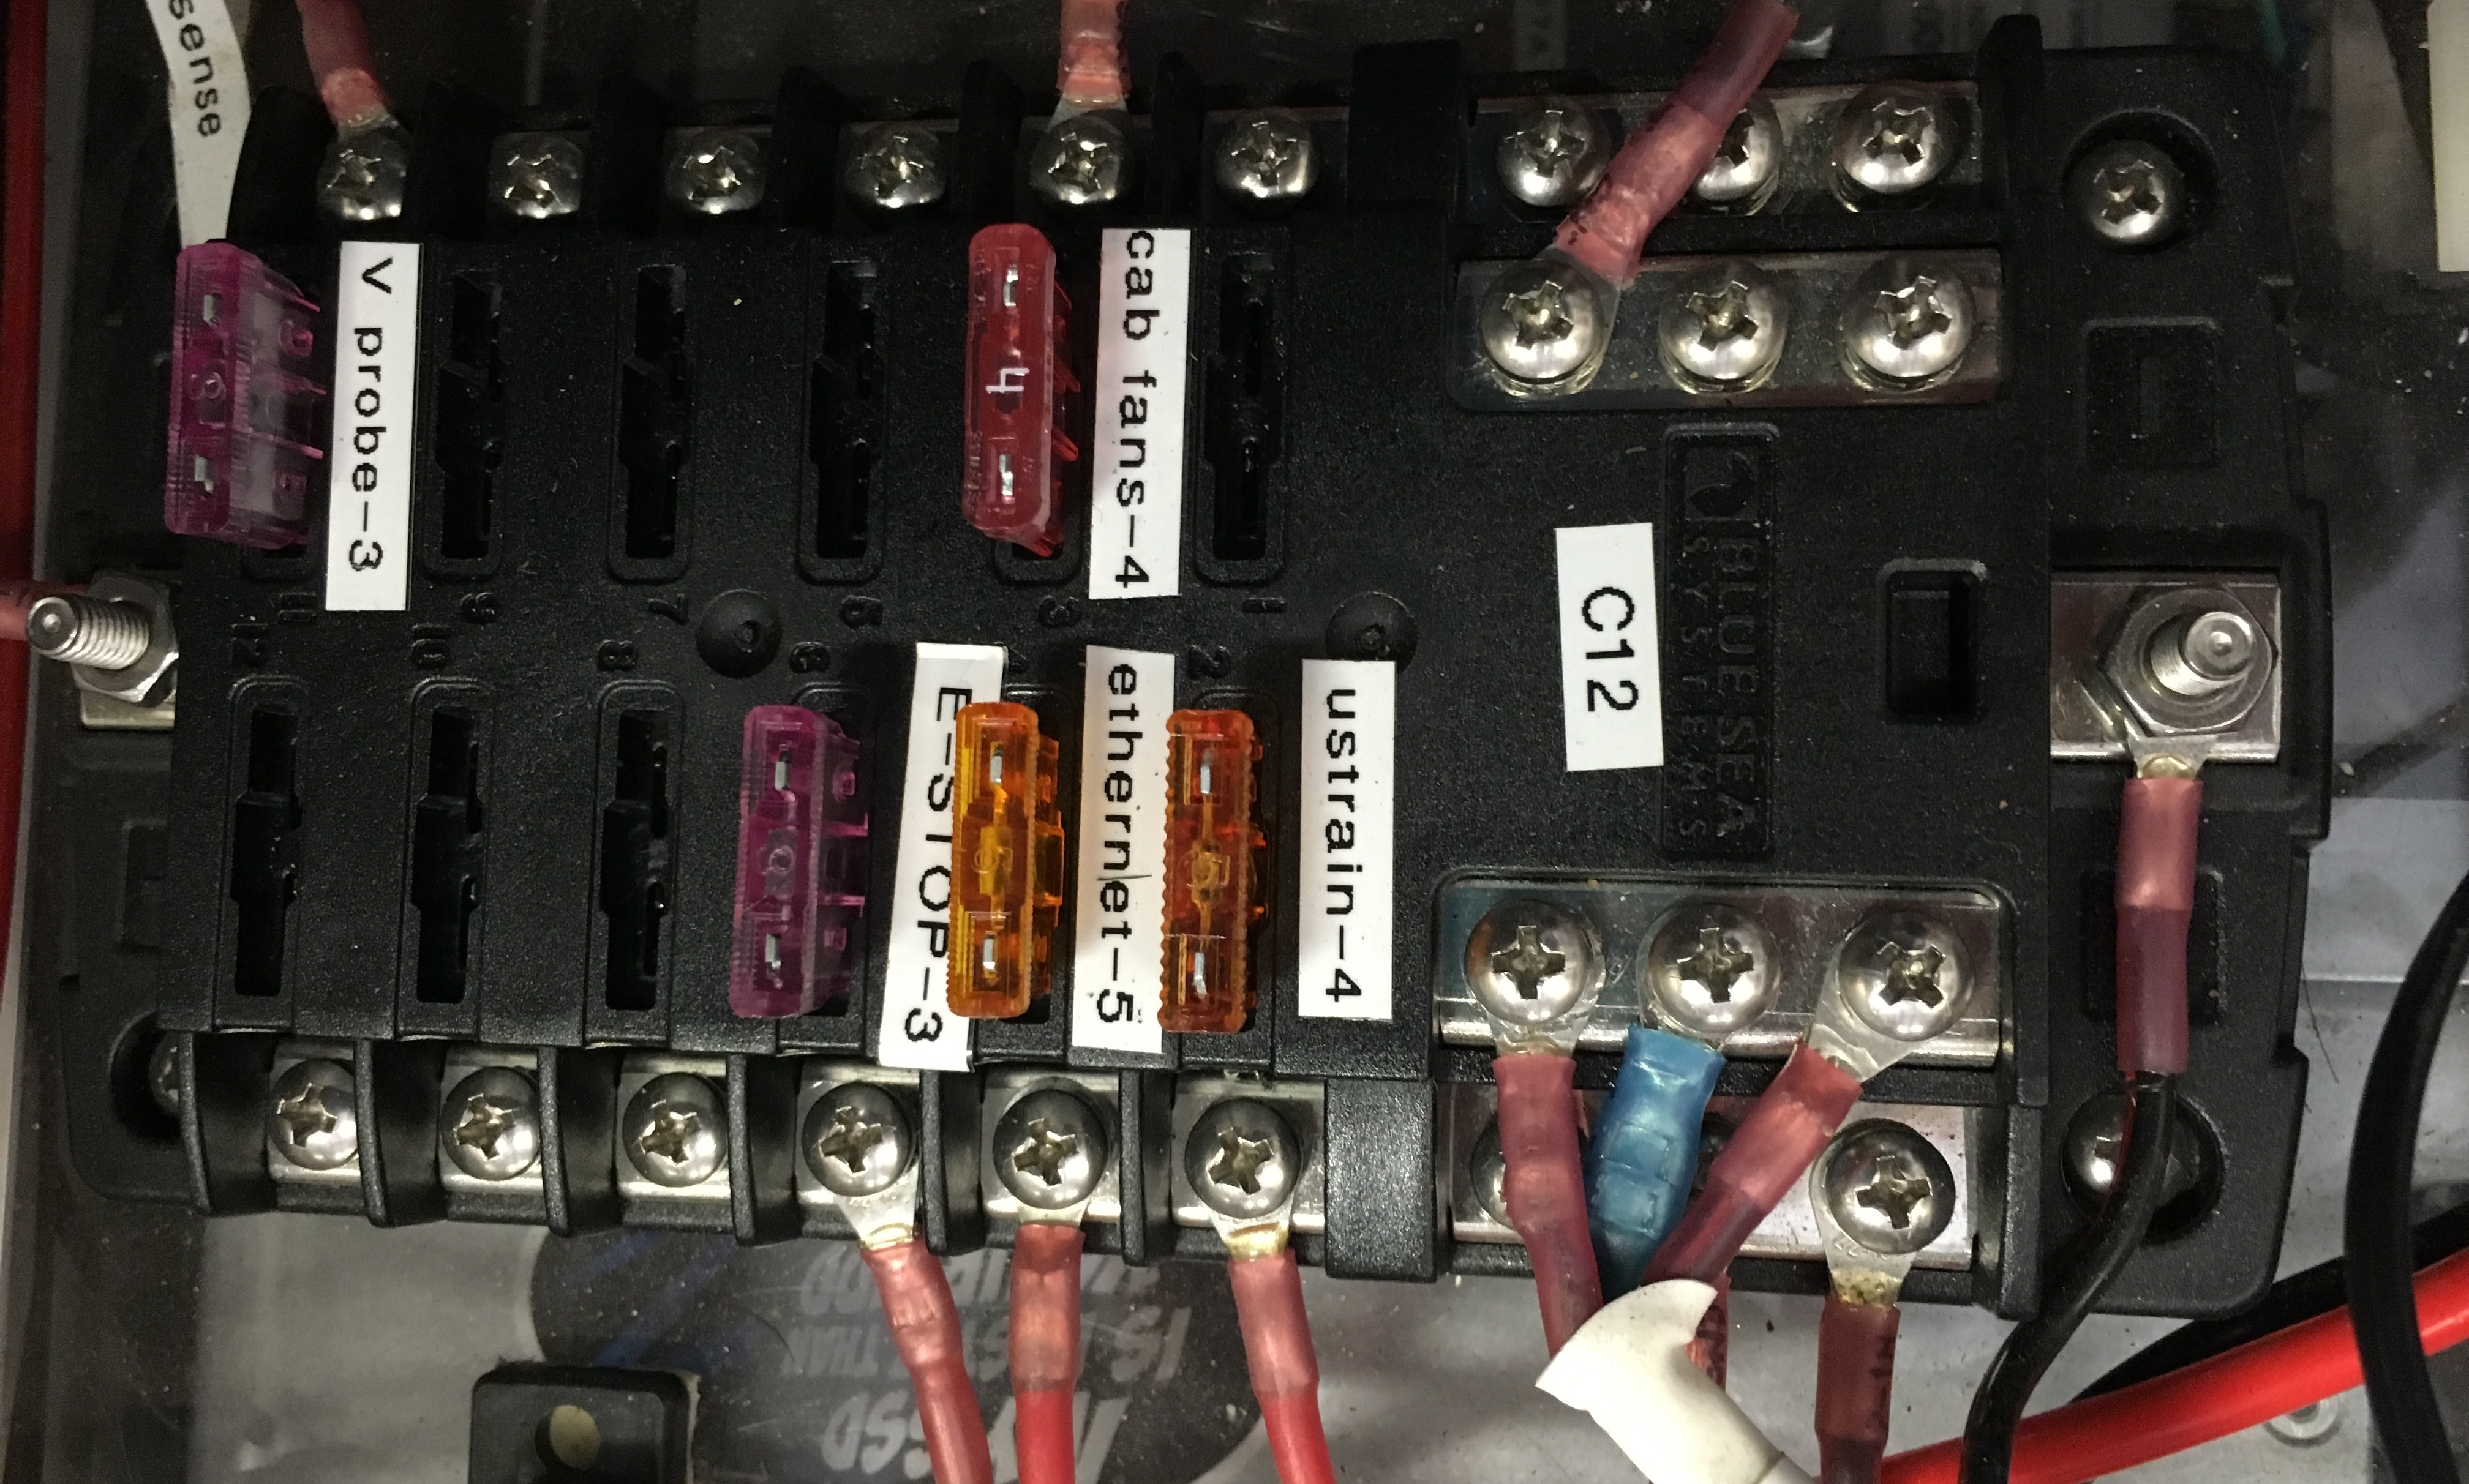
\includegraphics[scale=.06, angle=90]{Photos/C12.jpg}
\caption{\label{fig:C12} C12 Fuse Block}
\end{figure}
\end{minipage}

\bigskip

\noindent Power for the cab fans and INS power run to the appropriate equipment outside the electronics box. The signal to the 12V sensing probe runs to the voltage sense project box (discussed in a later subsection) and power to the ethernet switch runs to the netgear ethernet switch on the back corner of the electronics box on the driver's right side of the vehicle. The E-Stop 12V power is utilized by the E-Stop system, which will be discussed in a later section.

\subsubsection{12V Power Distribution (M12 Fuse Block)}

\begin{minipage}{0.6\textwidth}
All six outputs on the M12 fuse block are used:
\begin{enumerate}
\item Right tilt unit motor power
\item Power to the C12 fuse block
\item Power to the linear actuators
\item Left tilt unit motor power
\item Box fan power
\item Box fan power
\end{enumerate}
\end{minipage} \hfill
\begin{minipage}{0.5\textwidth}
\begin{figure}[H]
\centering
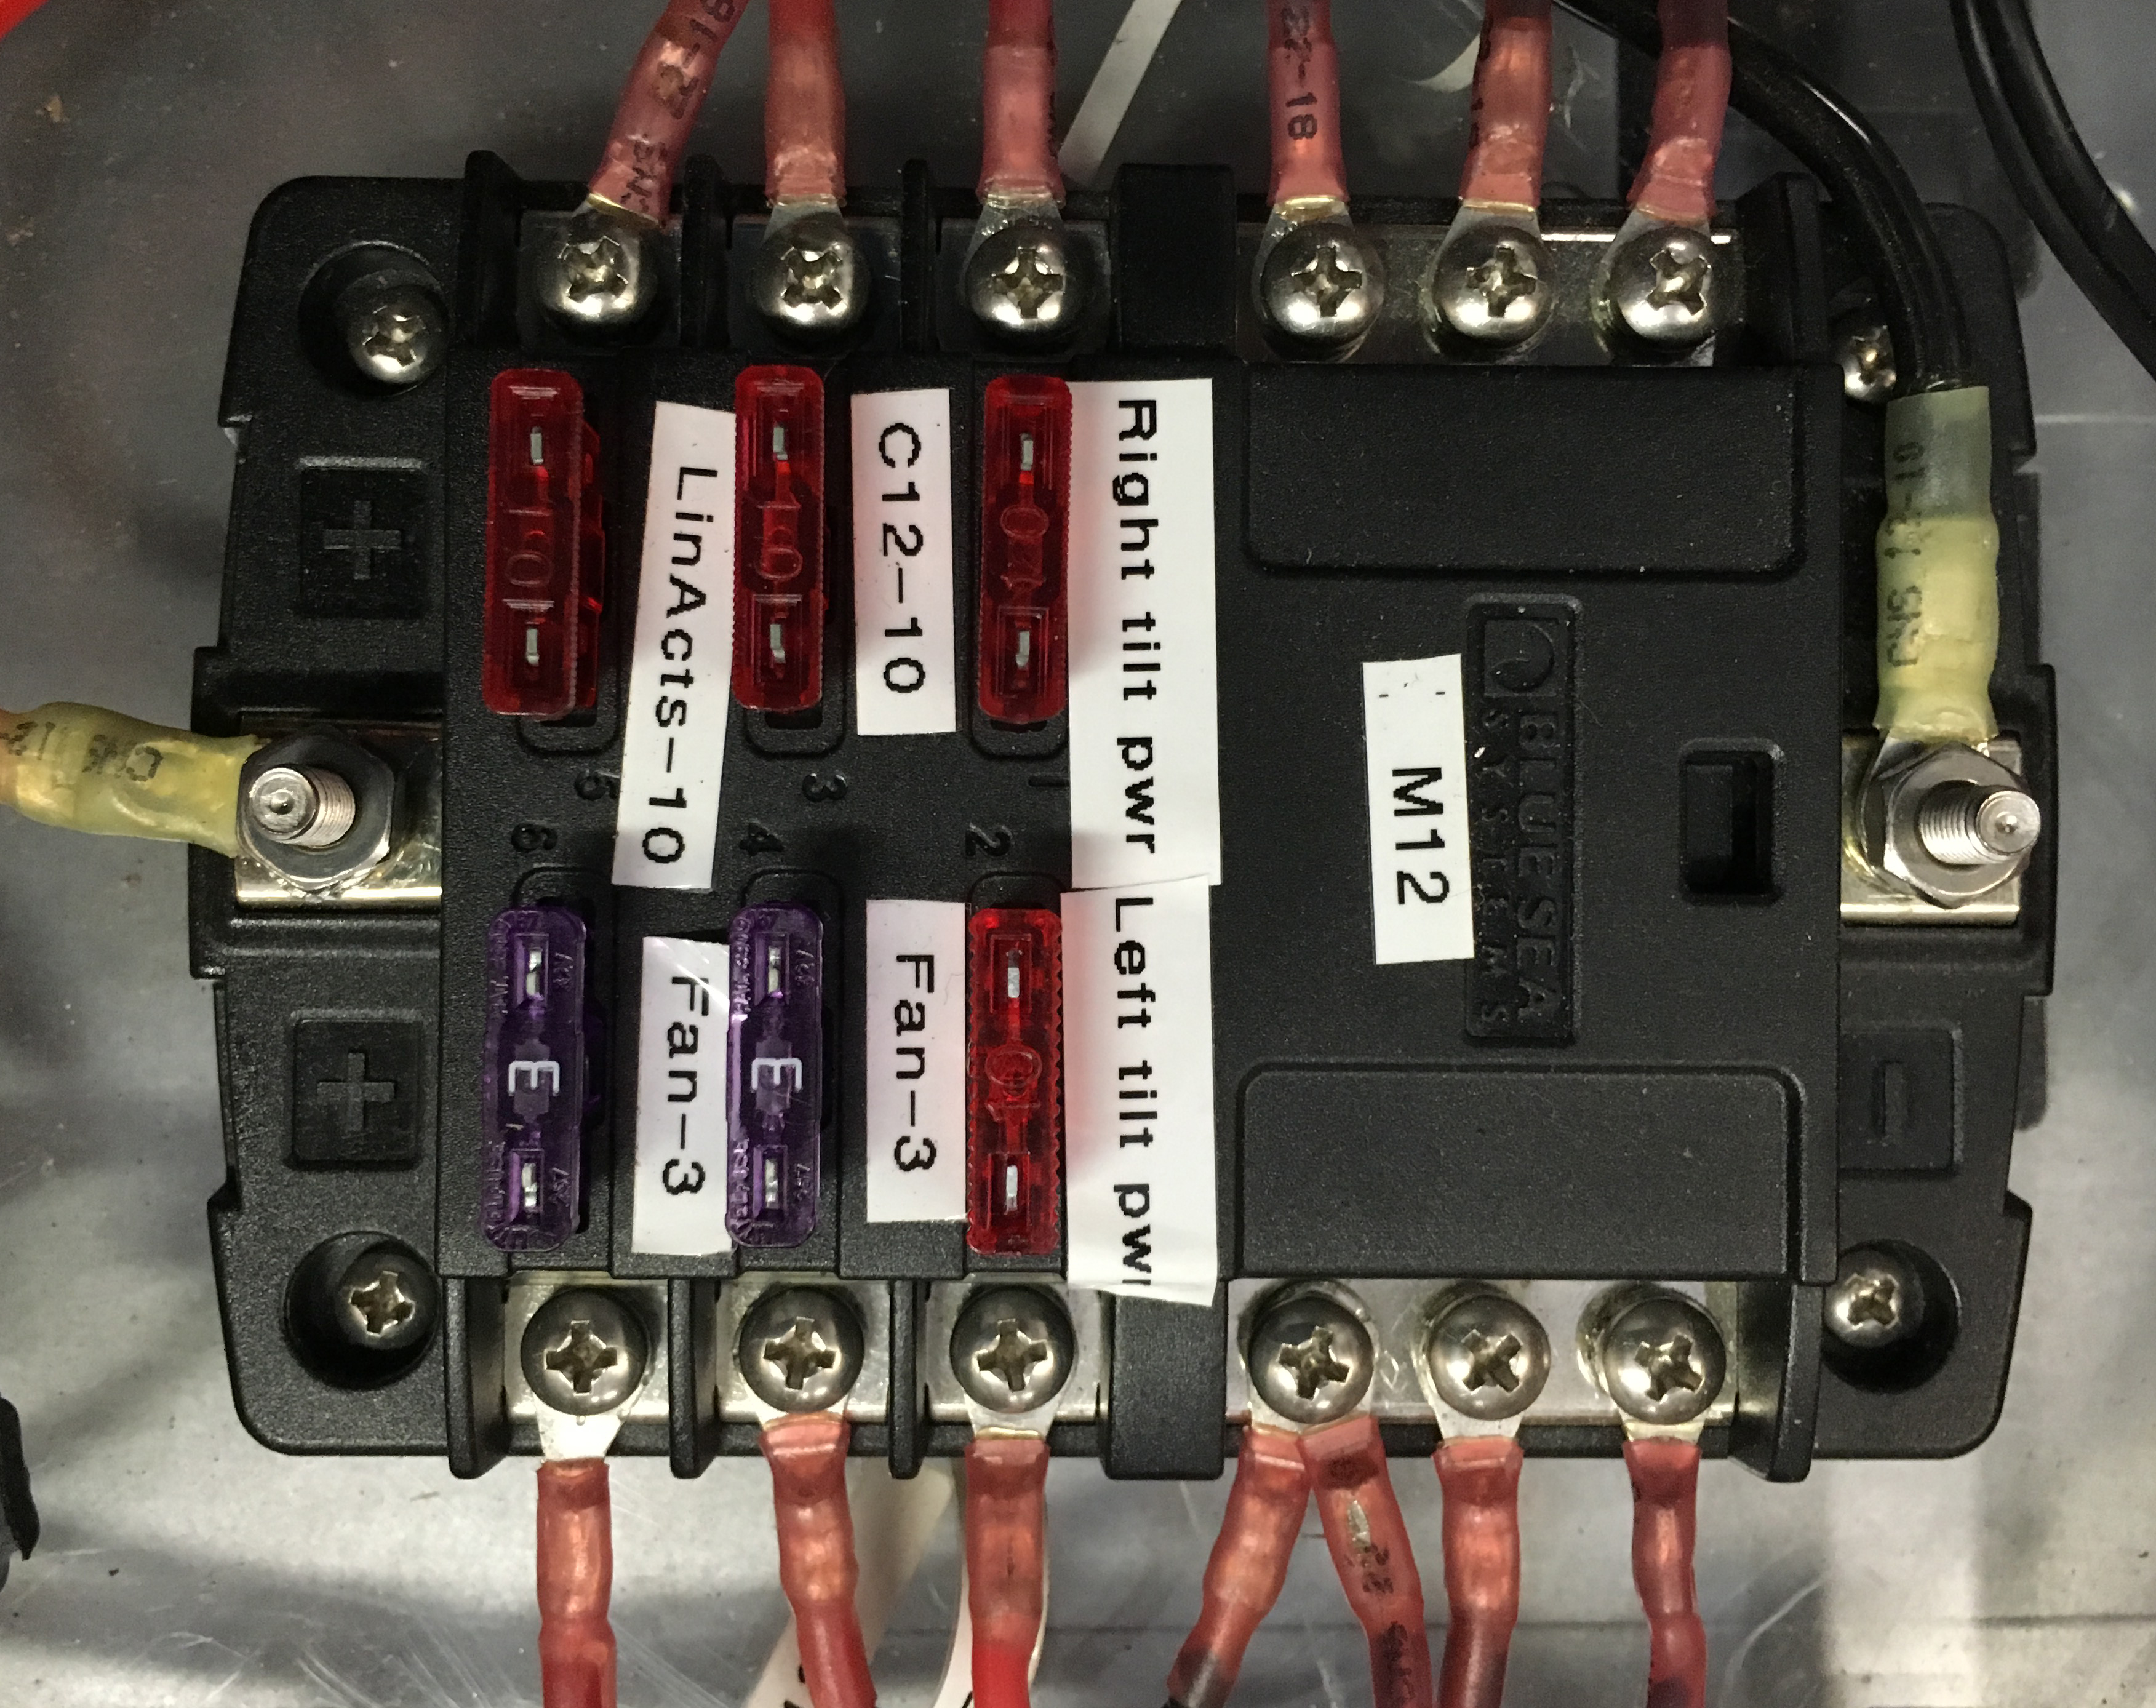
\includegraphics[scale=.06, angle=90]{Photos/M12.jpg}
\caption{\label{fig:M12} M12 Fuse Block}
\end{figure}
\end{minipage}

\bigskip

\noindent The power to the C12 fuse block is obtained from the appropriate port on the M12 fuse block. The power to each of the fans mounted to the front of the electronics box that cools the electronics box is also obtained from 2 of the outputs. Power to the right and left tilt units is also drawn from the M12 fuse block outputs and power then runs to the appropriate equipment outside the electronics box. Finally, the power for the linear actuators runs to an E-Stop relay first, then connected to two fuse terminals on the linear fuse block (discussed on the next page)

\subsubsection{Linear Fuse Block (Various Power Distribution)}

\begin{minipage}{0.6\textwidth}
The four lines on the linear fuse block are:
\begin{enumerate}
\item Fuse for motor power coming from the steering motor amplifier headed to the steering motor
\item Fuse for the 5V DC power output from the 5V DC power supply headed to the 5V DC power terminal strip
\item Two fuses to distribute 12V power from the E-Stop relay to the gas and brake linear actuators
\end{enumerate}
\end{minipage} \hfill
\begin{minipage}{0.5\textwidth}
\begin{figure}[H]
\centering
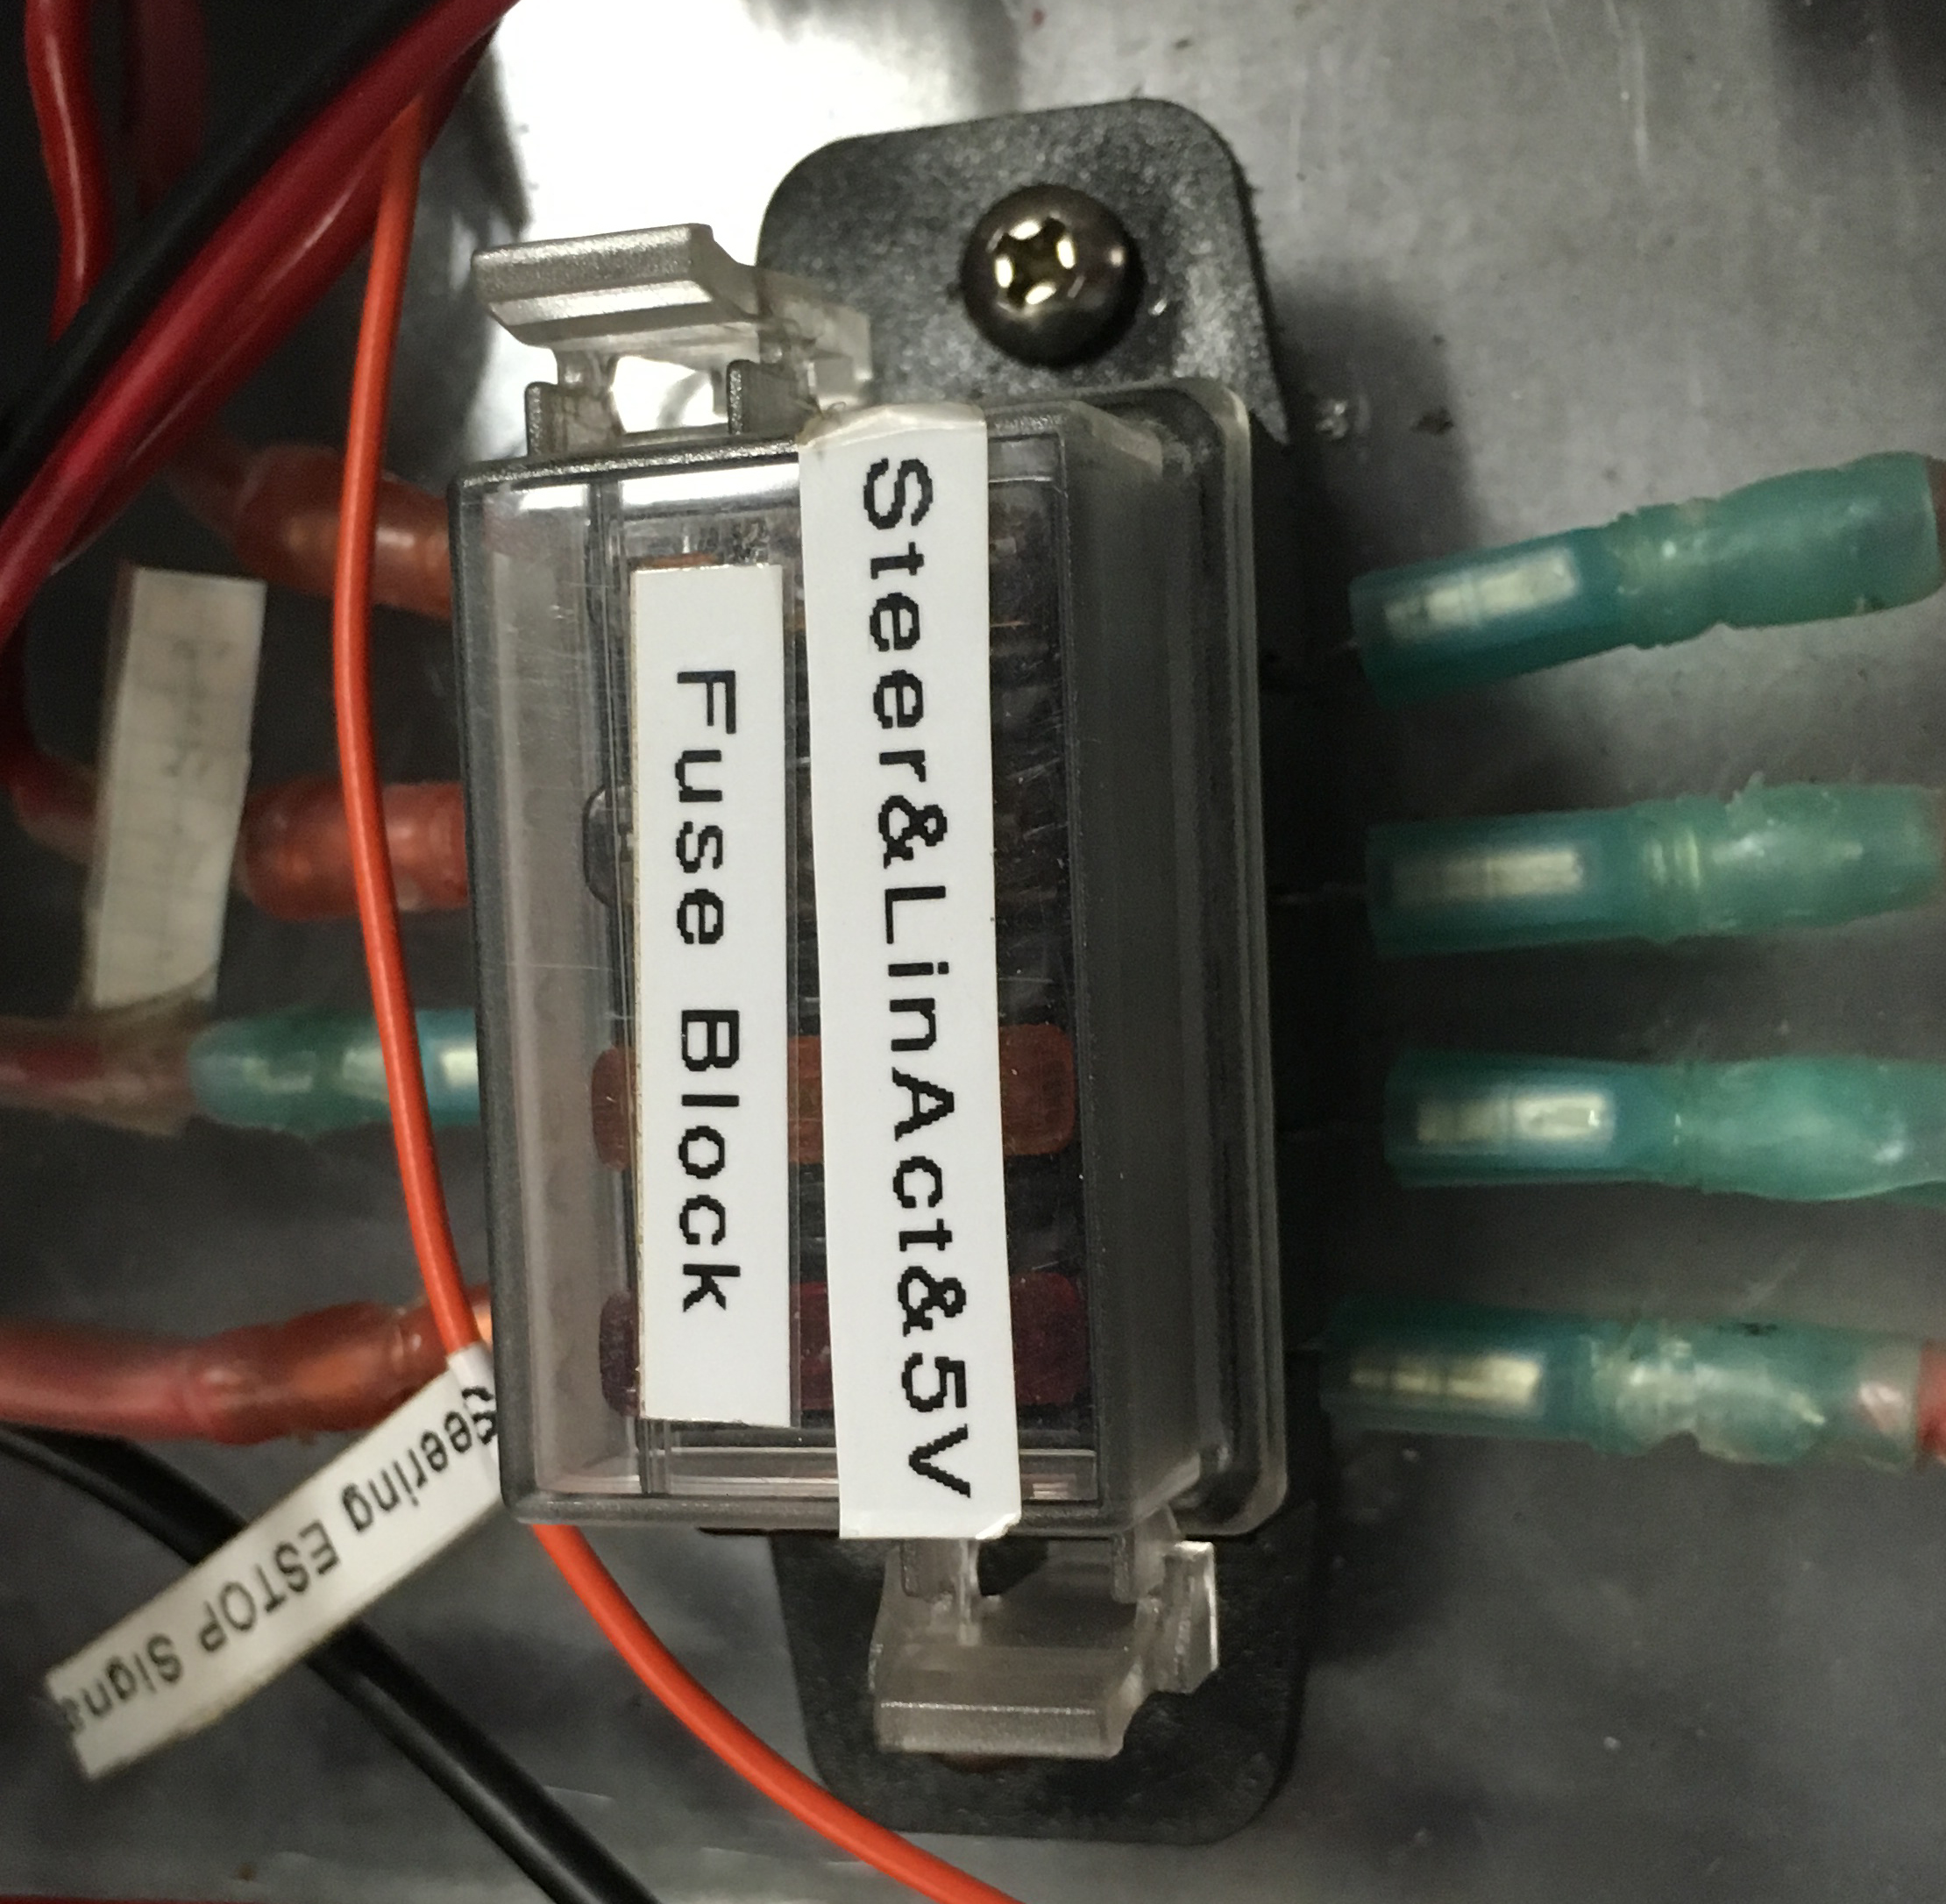
\includegraphics[scale=.06]{Photos/5vblock.jpg}
\caption{\label{fig:linear} Linear Fuse Block}
\end{figure}
\end{minipage}

\subsubsection{Terminal Strips (5V DC Power and Ground)}

There are two terminal strips that serve as busses for 5V DC power and ground.  The 5V DC power is used for:

\begin{enumerate}
\item Both commfronts that process serial signals from the LiDARs
\item To steering encoder
\item To cabin 5 volts
\item Signal to a 5V sensing probe
\end{enumerate}

\noindent The ground terminal strip is used for:

\begin{enumerate}
\item Ground connection for the E-Stop magnet coil
\item Ground to the 5V sensing probe
\item Ground to the E-Stop relay
\end{enumerate}

\newpage

\subsubsection{Emergency Stop System}

The emergency stop system is designed to mechanically cut power to the actuators in the event of an emergency. The last part of the power distribution system is the Emergency stop system. The system is relatively simple and consists of the following components:\\

\begin{enumerate}
\item 2 red mushroom-head emergency stop switches with black plastic mounting box, 1 located in the cab and one located on the outside wall of the electronics box
\item A magnecraft 788XBXM4L magnet coil relay with 70-463-1 relay socket located on the upper deck of the electronics box
\item The E-Stop sensing probe at the voltage sensing project box (discussed in the next section)
\end{enumerate}

\noindent The power source for the E-Stop system is a fused 12V terminal from the C12 fuse block. One branch of thsi line is then run through all the E-Stop switches. There is a second branch of this line that then runs to a relay on the upper deck of the electronics box. This relay controls power to the linear actuators and steering motor amplifier. When the E-Stops are not pressed, the line reads zero volts. When the E-Stops are pressed, the line is pulled up to 12V and that triggers the relay to open the normally-closed circuits and close the normally-open circuits, shutting down power to the linear actuators and disabling the steering motor amplifier.

\subsection{Subsystems and Signal Connections: Steering System}

The steering system is comprised of the following components:

\begin{enumerate}
\item Potomac Electric DC motor and steering encoder, which is an aftermarket power steering assist motor purchased by the 2009-2010 SCOPE team
\item Advanced Motor Controls 30A20AC analog servo drive with filter card
\item National Instruments NI9263 module that sends +/- 10V control signals to the analog servo drive
\item National Instruments NI9411 module that reads the steering encoder signals
\end{enumerate}

The 30A20AC analog servo driver and filter card are powered directly from the power strip on the side of the electronics box. The 30A20AC analog servo driver and filter card then used to drive the Potomac Electric DC motor. The steering encoder is powered via a 5 volt power line to the encoder.\\ \\
%
\noindent The 30A20AC analog servo driver takes PWM inputs and puts out motor voltage to the steering motor. In the LabVIEW FPGA code, the steering controller code communicates with the NI9263 module and uses the NI9263 module to output PWM control signals to the 30A20AC analog servo drive. Based on those PWM signals, the 30A20AC analog servo drive will then pass the appropriate motor voltage through the filter card before passing those signals to the Potomac Electric DC Motor mounted below the steering wheel. The steering encoder signals are read by the NI9411 module.

\subsection{Subsystems and Signal Connections: Gas and Brake Actuators}

The gas and brake pedal system consists of the following components:

\begin{enumerate}
\item 2 PQ Controls linear actuators, one for the brake ane and one for the gas pedal
\item National Instruments NI9263 chassis that sends analog control signals to the appropriate linear actuators
\end{enumerate}

The linear actuators share a common 12V power line that originates from the M12 fuse block. That power line is then split into two at the linear fuse block so that each linear actuator receives 12V power. \\ \\
%
\noindent The linear actuators accept anywhere between 1 - 4 volts and voltage corresponds linearly to position. Given that the linear actuators both have 3 inch strokes, the conversion should be 1 volt per inch of stroke. The voltage that controls the linear actuators is provided by the NI9263 chassis that is controlled by the FPGA code. 

\subsection{Subsystems and Signal Connections: LIDAR Serial Communication}

Serial communication with the left and right LIDARs on the front of the vehicle involves the following components:

\begin{enumerate}
\item 2 Sick LMLS291 LIDARs
\item 2 CommFront serial converters, one for each LIDAR
\item National Instruments NI9401 chassis that reads the serial lines
\end{enumerate}

Each LIDAR receives power from a terminal on the C24 fuse block. The CommFront serial converters are needed in order to convert the RS485 serial signal from the LIDARs to an RS232 signal that the NI chassis can interprete. After the CommFront serial converters, the signals are both fed into the NI9401 chassis to be read by the FPGA code.

\subsection {Subsystems and Signal Connections LIDAR Tilt Units}

The tilt unit system that nods the LIDARs consists of the following components:

\begin{enumerate}
\item 2 National Instruments NI9505 motor controller modules
\item 2 Bodine Electric DC Motors rated for HERP
\end{enumerate}

\noindent Unlike the steering system, the tilt unit system is driven entirely from the NI9505 motor controller modules. The modules themselves receive power from two sources: motor power for each module originates from a terminal on the C12 fuse block and connected to the input V+ and V- terminals on each module. The power for the controller electronics is received from the chassis itself. Each NI9505 motor controller module then drives its associated Bodine Electric motor by putting out power on the M+ and M- terminals. Each NI9505 motor controller module also handles the encoders for its associated tilt unit. The NI9505 motor controller module uses 5 pins on the serial connector on the module. 2 of the pins provide power and ground for each encoder and the other three pins handle the A, B and index outputs of the encoder. NEEDS SIGNAL DESCRIPTION?

 